\chapter{Lecture 15 Interpolation with Lagrange Polynomials}
\label{ch:lec15n}
\section{Objectives}
The objectives of this lecture are to:
\begin{itemize}
\item Discuss the problem of interpolation and illustrate how it can be done with linear least squares.
\item Introduce Lagrange polynomials as a preferable strategy for interpolation.
\item Illustrate the techniques with a MATLAB example.
\end{itemize}
\setcounter{lstannotation}{0}

\section{Interpolation with Least Squares}

Interpolation is a lot like curve fitting except that we expect the estimator to be \emph{exact} at the given data points.  In principle this can be done with linear least squares.  For any given $n$ data points, we can construct a polynomial interpolant of degree $n-1$ that matches the given data exactly.

\vspace{0.15cm}

\noindent \textbf{Example: } Create a 4\textsuperscript{th} order interpolant for the following 5 data points using linear least squares.

\begin{table}
\begin{tabular}{|c|c|c|c|c|c|}
\hline
$x$ & 1 & 4 & 7 & 10 & 13 \\ \hline
$y$ & 2 & 6 & 4 & 8 & 10 \\ \hline
\end{tabular}
\end{table}

\vspace{0.2cm} 

\noindent MATLAB code to carry out this process is provided in the listing below:
\marginnote[2.0cm]{

\noindent \ref{lst:ann15n-1} This is slightly tricky but the effect is to create a matrix, $X$, whose columns comprise $x^{n}$ for $n \in [0,1,2,3,4,5]$.

\vspace{0.25cm}

\noindent \ref{lst:ann15n-2} This is also tricky; note, in particular, that the $x$ in this line of code is different from the $x$ in the data section.  The effect is to create an interpolant of the form:
$$\text{nthInterp}(x) = c(1) + c(2)x^1 + \cdots c(n)x^{n-1}$$
}
\begin{lstlisting}[style=myMatlab]
clear
clc
close 'all'
% Data
x = [1 4 7 10 13]';
y = [2 6 4 8 10]';
% Create least squares interpolant
N = length(x);
X = x.^(0:N); /*!\annotation{lst:ann15n-1}!*/
c = (X'*X)\(X'*y);
nthInterp = @(x) (x.^(0:N))*c; /*!\annotation{lst:ann15n-2}!*/
\end{lstlisting}

\noindent The data and least squares interpolant are presented in Figure \ref{fig:lec15n-ex-ls-interp}.  
\begin{marginfigure}
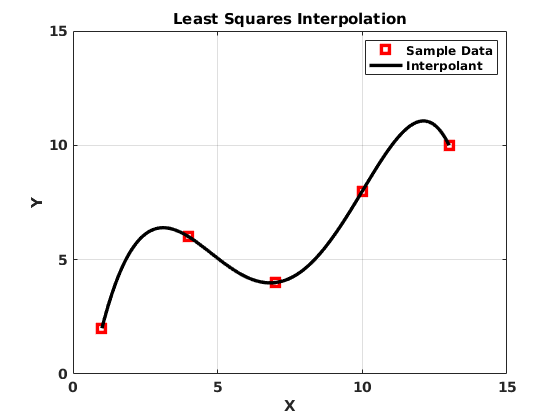
\includegraphics{lec15n-ex-ls-interp.png}
\caption{Least squares interpolation of data points.}
\label{fig:lec15n-ex-ls-interp}
\end{marginfigure}
Notice that, while the interpolant---as required---manages to pass through all of the data points, it is not an altogether great representation of the overall trend of the data.\sidenote{I suspect that  you would not want to really use this interpolant to estimate values between the data points.} Some other problems that are inherent to this approach:
\begin{enumerate}
\item As $n$ increases, the columns of \lstinline[style=myMatlab]{X} are more ``like'' each other.  As a result, the condition number of \lstinline[style=myMatlab]{(X'*X)} increases and, as we learned in Lecture 10, there is as a consequence greater numerical error in solving the linear system to find the coefficients.  In fact, when I execute this code in MATLAB, an error is issued due to the high condition number of \lstinline[style=myMatlab]{(X'*X)}:

\begin{figure}
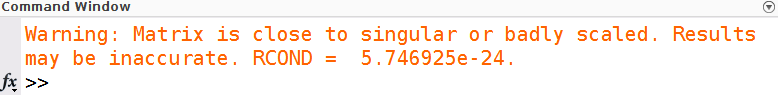
\includegraphics[width=0.75\textwidth]{lec15n-ex-ls-interp-warn.png}
\caption{Warning issued by MATLAB due to the high condition number of \lstinline[style=myMatlab]{(X'*X)}.}
\label{fig:lec15n-ex-ls-interp-warn}
\end{figure}

\item Solving a set of linear equations for the interpolating coefficients is inconvenient for some applications.  Working in a MATLAB environment we might forget that, generally speaking, solving a linear system of equations is complicated. 
\end{enumerate}

\noindent For applications later in the course, such as finite element methods, we will be very picky about the quality of interpolation functions and we will not be particularly interested in solving systems of linear equations on each domain that we hope to use such interpolations.  Luckily, there are better methods that avoid both of these problems.

\section{Lagrange Polynomial Interpolation}

Suppose we have 3 data points---$x_1$, $x_2$, and $x_3$---and we want to derive a 2\textsuperscript{nd} order polynomial interpolant, and we specify the polynomial as follows:
\begin{equation*}
f(x) = y = a_1(x-x_2)(x-x_3) + a_2(x-x_1)(x-x_3) + a_3(x-x_1)(x-x_2)
\end{equation*}
Notice the form of this polynomial; when we evaluate $f(x)$ at $x_1$, the first term on the right is the only non-zero term; when we evaluate $f(x_2)$, only the second term on the right is non-zero and similarly for when we evaluate $f(x_3)$.  This makes it easy to find values for $a_1$, $a_2$ and $a_3$.  Since
\begin{align*}
f(x_1) &= y_1 \\
&=a_1(x_1 - x_2)(x_1 - x_3) + a_2 \cancelto{0}{(x_1 - x_1)}(x_1 - x_3) + a_3\cancelto{0}{(x_1 - x_1)}(x_1 - x_2) \\
\Rightarrow a_1 &= \frac{y_1}{(x_1 - x_2)(x_1 - x_3)} 
\end{align*}
We can derive equations for $a_2$ and $a_3$ in the same way:
\begin{align*}
a_2 & = \frac{y_2}{(x_2 - x_1)(x_2 - x_3)} \\
a_3 & = \frac{y_3}{(x_3 - x_1)(x_3 - x_2)}
\end{align*}

\noindent Thus we have specified, what we will call, a Lagrange polynomial through these points:
\begin{equation*}
f(x) = \frac{(x - x_2)(x - x_3)y_1}{(x_1 - x_2)(x_1 - x_3)} + \frac{(x - x_1)(x-x_3)y_2}{(x_2 - x_1)(x_2 - x_3)} + \frac{(x - x_1)(x-x_2)y_3}{(x_3-x_1)(x_3 - x_2)}
\end{equation*}
In general, we construct the Lagrange polynomial as shown in Equation \ref{eq:lec15n-lagrange}:
\begin{equation}
f(x) = \sum\limits_{i=1}^{n} y_i L_i(x) = \sum\limits_{i=1}^{n} y_i \underbrace{\prod_{\substack{j=1 \\ j \ne i}}^{n} \frac{(x - x_j)}{(x_i - x_j)}}_{\substack{\text{Lagrange} \\ \text{function}}}
\label{eq:lec15n-lagrange}
\end{equation}
While this formulation avoids the aforementioned problems, it still can result in a low-quality interpolant.  It turns out that the quality of the interpolant depends on the number of points one hopes to interpolate and \emph{the spacing} of these points.  In particular, uniformly spaced interpolating points results in low quality interpolants.

Consider, as an example, following function:
\begin{equation*}
f(x) = \frac{8a^3}{x^2 + 4a^2}
\end{equation*} 
where $a$ is a parameter.  This is the so-called Witch of Agnesi\cite{WOA} problem and it is a classic test case for interpolation schemes.\cite{trefethen2} If we set $a=0.15$ and construct a Lagrange interpolant with uniformly spaced points, we get the result shown in Figure \ref{fig:lec15n-woa-uniform}.  The interpolation improves as $n$ increases everywhere except near the endpoints of the domain.  At the endpoints, the interpolation becomes worse.

%\begin{fullwidth}
\begin{figure}
\subfloat[]{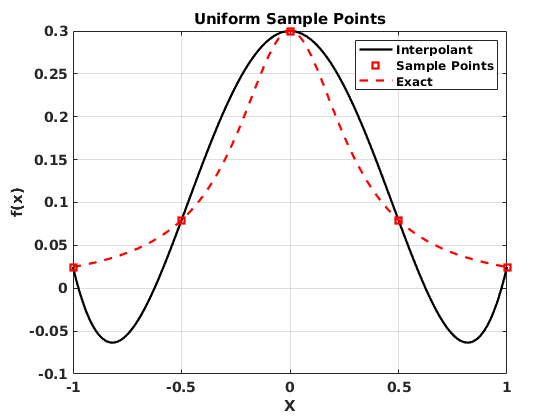
\includegraphics[width=2.25in]{lec15n-ex2-u-n5.png}}
\subfloat[]{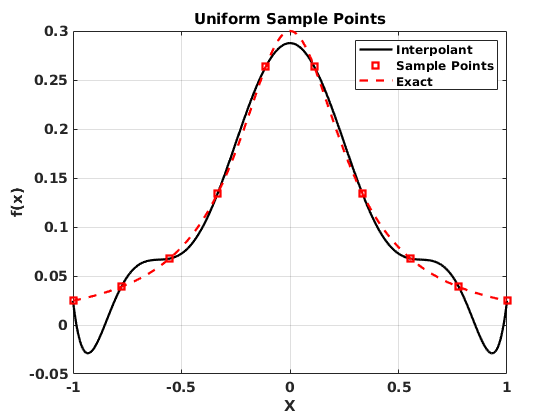
\includegraphics[width=2.25in]{lec15n-ex2-u-n10.png}}
\\
\subfloat[]{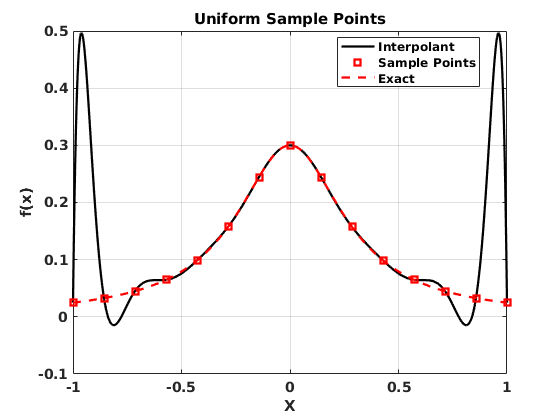
\includegraphics[width=2.25in]{lec15n-ex2-u-n15.png}}
\subfloat[]{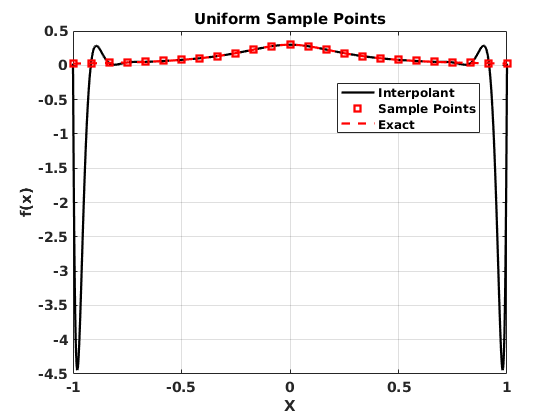
\includegraphics[width=2.25in]{lec15n-ex2-u-n25.png}}
\label{fig:lec15n-woa-uniform}
\caption[][0.0cm]{Lagrange interpolation with $n=5$, $n=10$, $n=15$, and $n=20$ uniformly spaced points.}
\end{figure}
%\end{fullwidth}
If instead of using uniformly spaced points, we choose particular set of non-uniformly spaced points, the quality of the interpolation is much improved.  In Figure \ref{fig:lec15n-woa-cheb} we select \emph{Chebyshev nodes} for interpolation.\sidenote{Chebyshev nodes, on the interval $x\in[-1,1]$ are given by:
$$x_k = \cos{\left(\frac{2k - 1}{2n}\pi \right)}, \ k=1,\dots,n$$
or for an arbitrary interval $x \in [a,b]$ via the following mapping:
$$x_k = \frac{1}{2}(a+b) + \frac{1}{2}(b-a)\cos{\left(\frac{2k - 1}{2n}\pi \right)}, \ k=1,\dots,n$$
} 
\begin{figure}
\subfloat[]{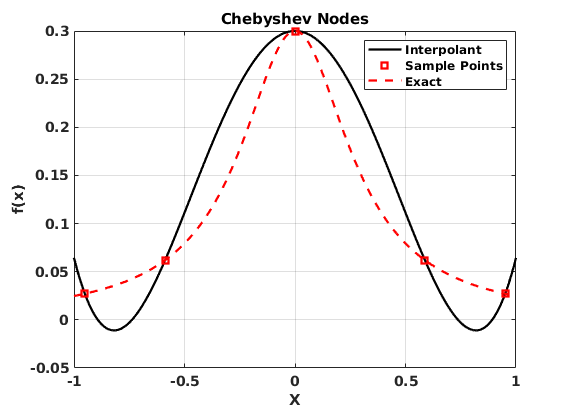
\includegraphics[width=2.25in]{lec15n-ex2-c-n5.png}}
\subfloat[]{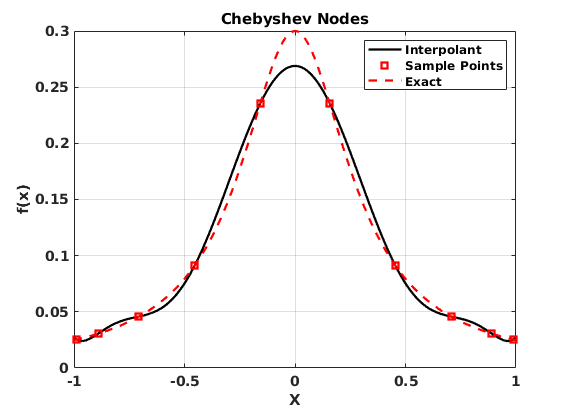
\includegraphics[width=2.25in]{lec15n-ex2-c-n10.png}}
\\
\subfloat[]{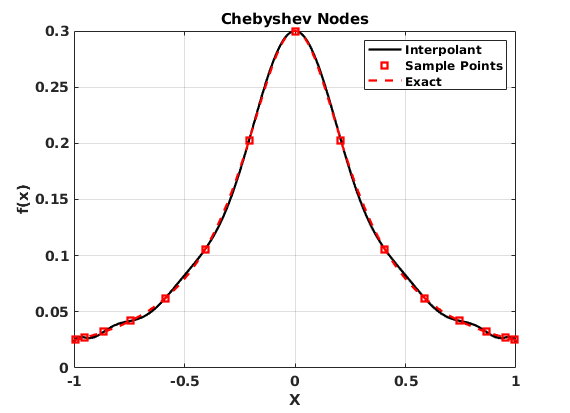
\includegraphics[width=2.25in]{lec15n-ex2-c-n15.png}}
\subfloat[]{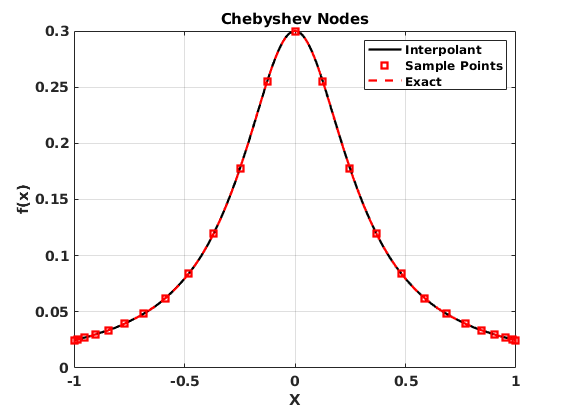
\includegraphics[width=2.25in]{lec15n-ex2-c-n25.png}}
\label{fig:lec15n-woa-cheb}
\caption[][0.0cm]{Lagrange interpolation with $n=5$, $n=10$, $n=15$, and $n=20$ points placed at Chebyshev nodes.}
\end{figure}
To be sure, there are many contexts in which the analyst, who is devising the interpolation scheme, is not at liberty to choose the sample points. In cases where you can choose the sample points, know that how you choose your points makes a difference.

\section{Matlab Example}
In this example, we will illustrate a case where the user does \emph{not} have a choice in the sample points.  Nonetheless, it will be worthwhile to show the MATLAB code so you can adapt it to a case of interest to you.

We will start by clearing out the workspace and loading the data we wish to interpolate.
\begin{lstlisting}[style=myMatlab,name=lec15n-ex2]
clear
clc
close 'all'

%% Load data
Strain = [0 0.4 0.8 1.2 1.6 2.0 2.4 2.8 3.2...
    3.6 4.0 4.4 4.8 5.2 5.6 6.0]';% dimensionless
Stress = [0 3.0 4.5 5.8 5.9 5.8 6.2 7.4 9.6...
    15.6 20.7 26.7 31.1 35.6 39.3 41.5]'; % MPa
\end{lstlisting}

Once the data is defined, we can create interpolations with both monomials and Lagrange polynomials.  

\begin{lstlisting}[style=myMatlab,name=lec15n-ex2]
%% N-th order Interpolation (monomials)

N = length(Strain);
X = Strain.^(0:N);
c = (X'*X)\(X'*Stress);
nthInterp = @(x) (x.^(0:N))*c;

%% Lagrange Interpolation
F = genLagrangePolyInterp(Strain,Stress);
\end{lstlisting}

Of course, all of the work for the Lagrange polynomial interpolation is packaged into the local function \lstinline[style=myMatlab]{genLagrangePolyInterp(X,Y)}.  The MATLAB code to make that happen is shown next.

\begin{lstlisting}[style=myMatlab,name=lec15n-ex2]
%% Local function for Lagrange polynomial
function F = genLagrangePolyInterp(X,Y)
% function F = genLagrangePoly(X,Y) generates a Lagrange  
% polynomial that may be used to interpolate a function
% inputs
% X = x-values of a function
% Y = f(X) for some function
%
% Outputs
% F - a function handle with the Lagrange interpolant

n = length(X); 

F = @(x) 0; % initialize the interpolant

for i = 1:n
    L = @(x) Y(i); % initialize the Lagrange Function
    for j = 1:n
        if j ~= i
            L = @(x) L(x).*((x - X(j))./(X(i) - X(j)));
        end
    end
    F = @(x) F(x)+L(x);
end
end
\end{lstlisting}

We can plot the resulting interpolants; these are shown in Figure \ref{fig:lec15n-ex3-monomial} and Figure \ref{fig:lec15n-ex3-lagrange} for monomial and Lagrange interpolation respectively.  As can be seen, the Lagrange interpolant is not great.  Nonetheless, the use of Lagrange polynomials for interpolation is a valuable tool, particularly for cases where the analyst can select the sample points for the interpolant.
\begin{marginfigure}
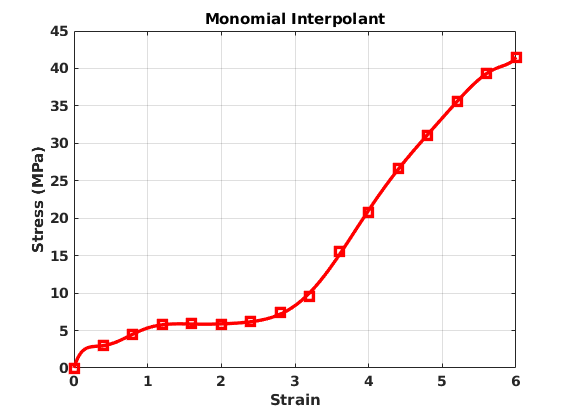
\includegraphics{lec15n-ex3-monomial.png}
\caption{Monomial interpolant for stress-strain data.}
\label{fig:lec15n-ex3-monomial}
\end{marginfigure}

\begin{marginfigure}
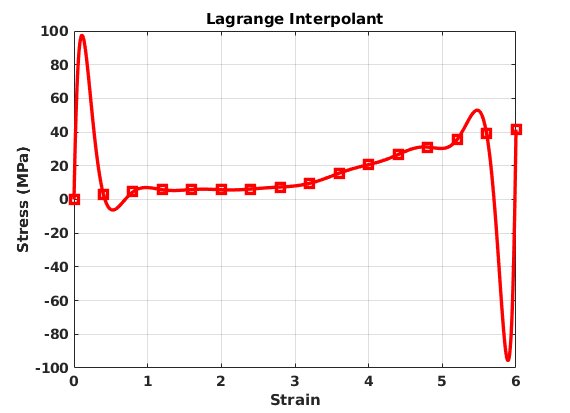
\includegraphics{lec15n-ex3-lagrange.png}
\caption{Lagrange interpolation for stress-strain data.}
\label{fig:lec15n-ex3-lagrange}
\end{marginfigure}

